\chapter{Introduction} 

\section{Background}

\subsection{Mobile Ad Hoc Networks}
A mobile ad hoc network (MANET),  is a self-configuring mobile mesh network of mobile devices connected by wireless links.  
These mobile devices are free to move independently in any direction and it acts as a router, where it must forward traffic unrelated to its own use. 

\subsection{Highly Partitioned Networks}
Highly partitioned networks are networks with no single hop or multiple hop route between some or even all node pairs.

\subsection{Store Carry Forward \& Message Ferrying}
Some messages are dropped if no route to the destination can be found.  
Message ferrying allows the message to buffer and carry messages until the connection is available to forward.

\section{Motivations and Potential Applications}

With the continuous growth of today's mobile devices, such as smartphones, laptops, tablets, netbooks, and more, demands for different services are prominent. 
%The idea is to implement integrated intelligence for networked machine monitoring and controlling.
Some of these applications are integrated intelligence for networked monitoring and controllability between machines, track road traffic conditions, in-house utility management, automation for home devices, industrial monitoring applications, robot to robot communication and more.  
The use of these mesh networks must have low-cost, very low power consumption,low data rate, cheap installation, flexibility, and increase connectivity to make it worthwhile in most cases.


\section{Project Goals}
Research and implement a mesh network design with varying distances using ZigBee protocol and examine the feasibility for different applications.


%testingstuff
\section{Section 1}
\label{sec:sec-1}

Citation ~\cite{book1}.
Reference to section 1: \ref{sec:sec-1}




An overview look of our architecture:

\begin{figure}[h]
    \centering
    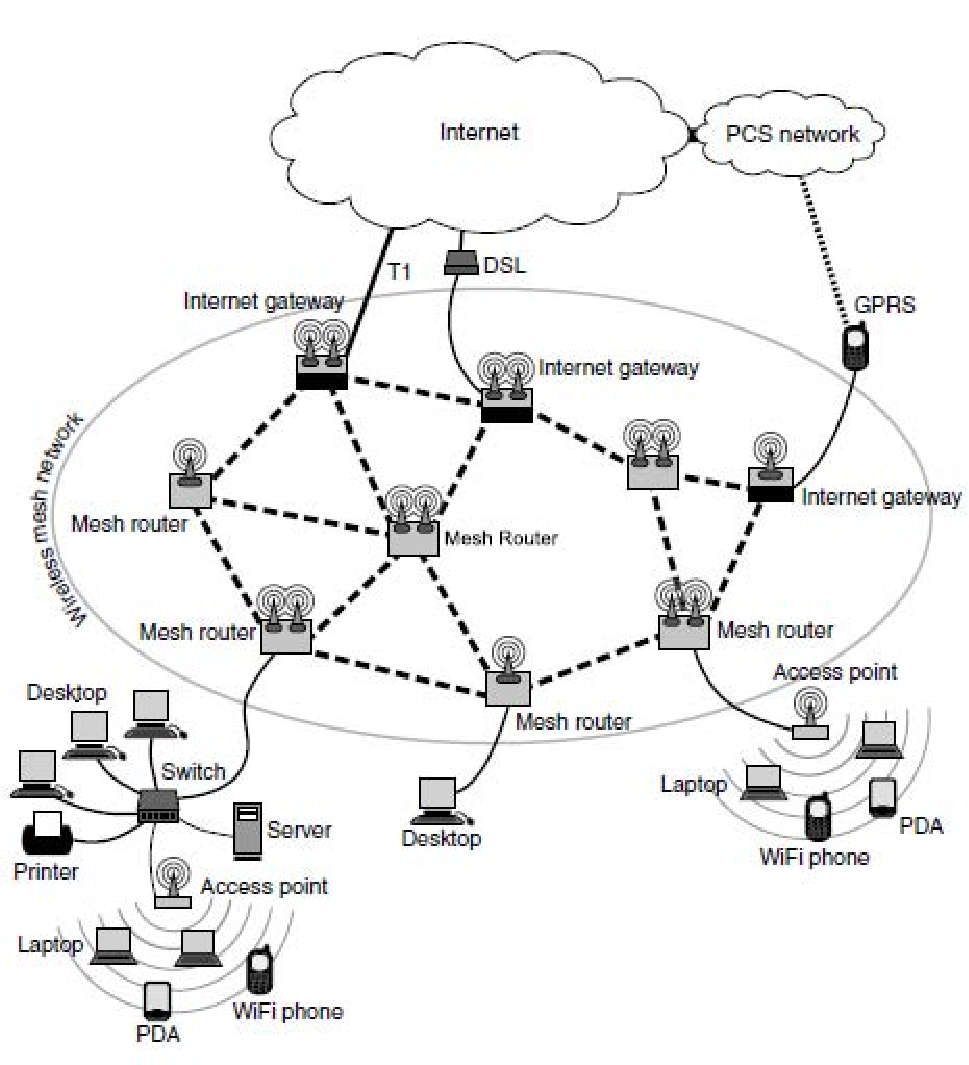
\includegraphics[width=.5\textwidth]{images/wmn_general}
    \caption{Wireless Mesh Network General Architecture Overview~\cite{book1}}
    \label{fig:wmn_general}
\end{figure}

if something referring to this figure, use this \ref{fig:wmn_general}


Testing; just making references show
asdf ~\cite{wearable}.
asdf ~\cite{adhocmsgferry}.
asdf ~\cite{hybrid}.
asdf ~\cite{QoSrouting}.
asdf ~\cite{efficientrouting}.
asdf ~\cite{implement}.
asdf ~\cite{book1}.
